\section{Grundlagen}
\label{sec:Grundlagen}
Seit der ersten theoretischen Beschreibung der stimulierten Emission von Albert Einstein 1916 und dem experimentelle Beweis 1928 von Rudolf Ladenburg wurde der Laser stets weiterentwickelt. Die Anwendungsmöglichkeiten beschränken sich nicht nur auf die verschiedensten Zweige der Wissenschaft sondern finden ebenfalls Verwendung im Alltag. Der letzte große Erfolg wurde 2018 mit einem Nobelpreis ausgezeichnet, da es gelang mit Hilfe eines Lasers eine optische Pinzette zu realisieren.

In den folgenden Kapitel wird zunächst auf die Grundlagen und die essenziellen Bestandteile einen Lasers eingegangen, gefolgt von der Beschreibung des Diodenlasers. Anschließend erfolgt eine Beschreibung der bei der Durchführung vorgenommenen Schritte.

\subsection{Laser}
Wird ein System angeregt, kehrt es nach einer gewissen Zeit in seinen Grundzustand zurück. Der Energieunterschied zwischen den beiden Zuständen wird bei der Rückkehr in den Grundzustand in Form eines Photons oder eines Phonons ungewandelt, welches emittiert wird. Die Emission eines Photons kann dabei spontan oder stimuliert entstehen. Der spontane Übergang in ein niedrigeres Niveau ist ein zufälliger, ungetriebener Prozess. Die stimulierte Emission wird Gegensatz dazu, durch ein externes Photon ausgelöst. Weißt dieses Photon genau die Energie der Energiedifferenz zwischen zwei Niveaus auf, geht das System in das niedrigere Niveau über und emittiert dabei ein Photon gleicher Wellenlänge und Phase. Den Zustand, das sowohl die Wellenlänge als auch die Phase übereinstimmen, wird als Kohärenz bezeichnet und ist die Grundlage jedes Lasers.

\subsubsection{Bestandteile}
\label{sec:Bestandteile}
Jeder Laser benötigte für eine erfolgreiche kohärente Emission im wesentlichen eine Pumpen, ein aktives Medium, einen Resonator und eine Kühlung.

Die Pumpe regt im Grundzustand befindliche Elektronen an, die dadurch in einen angeregten Zustand übergehen. Die Elektronenverteilung wird dabei über die Fermifunktion
\begin{align}
	f(E)=\frac{1}{e^{\frac{E-\mu}{k_B T}}+1}
\end{align}
beschrieben. Diese ist Abhängig von der Energie der Elektronen $E$, dem chemischen Potential $\mu$, der Bolzmannkonstante und der Temperatur $T$ des Systems. Bei fallender Temperatur gehen somit immer mehr Elektronen in den Grundzustand über, bis der Grenzfall erreicht ist und ausschließlich der Grundzustand besetzt ist. Im gegenteiligen Grenzfall konvergiert die Funktion gegen $1/2$, wodurch der angeregte Zustand als auch der Grundzustand gleich besetzt sind. Der beschriebene Verlauf ist in Abbildung \ref{sze1} dargestellt.

\begin{figure}[H]
\centering
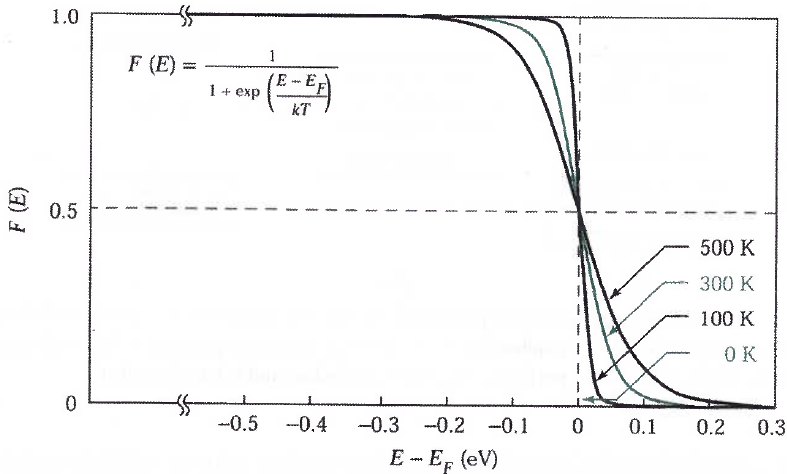
\includegraphics[width=0.7\textwidth]{ressources/fermi.png}
\caption{Darstellung der Fermiverteilung für verschiedene Temperaturen. \cite{SZE}}
\label{sze1}
\end{figure}


Für die zuvor angesprochene stimulierte Emission muss eine Besetzungsinversion realisiert werden. Dieses ist in einem System mit drei oder mehr Energieniveaus möglich. Dabei, wie in Abbildung \ref{theo1} angedeutet, erfolgt die Relaxation in das zweite Energieniveau wesentlich schneller als die Relaxation vom zweiten in das erste Niveau. 


\begin{figure}[H]
\centering
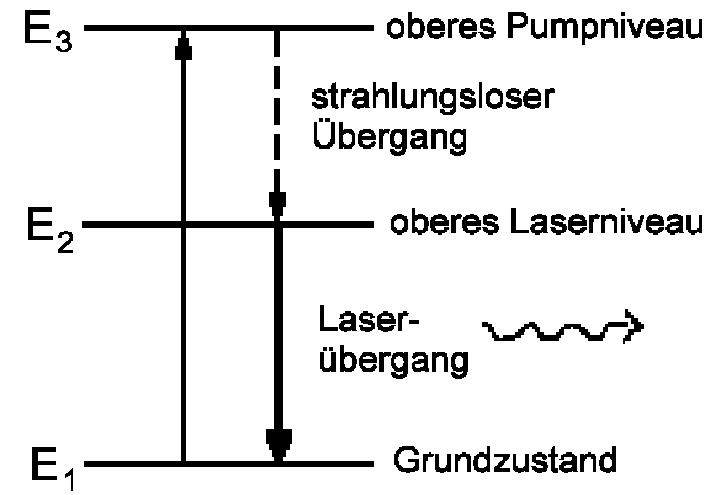
\includegraphics[width=0.5\textwidth]{ressources/Niveau.jpeg}
\caption{Darstellung eines Drei-Niveau-Systems. \cite{skript}}
\label{theo1}
\end{figure}


Somit befindet sich ein Großteil der Elektronen im zweiten Niveau, wodurch die geforderte Besetzungsinversion realisiert wird. Die Spiegel, die das aktive Medium einschließen, bilden den sogenannten Resonator und reflektieren die entstanden Photonen. Die stehende Wellen im Resonator müssen die folgenden Bedingungen erfüllen:
\begin{align}
	\lambda=\frac{2Ln}{m}\qquad \text{und} \qquad\nu=\frac{cm}{2Ln}\:, \quad \text{mit}  \quad m \in \mathbb{N} 
\end{align}
Zwischen den verstärkten Frequenzen besteht ein äquidistanter Abstand von
\begin{align}
	\Delta \nu=\frac{c}{2Ln}.
\end{align}
Für den Grenzfall $\nu >>\Delta\nu$ besteht ein proportionaler Zusammenhang zwischen der Wellendifferenz
\begin{align}
	\Delta \lambda =\lambda_2- \lambda_1=c\left(\frac{1}{\nu_2}-\frac{1}{\nu_1}\right) \approx \frac{c}{\nu^2}\Delta\nu.
	\label{eq:1}
\end{align}
und dem Frequenzunterschied. Einer der verwendeten Spiegel reflektiert nur etwa $\SI{95}{\percent}$ der einfallenden Photonen, wodurch der entstandene Laserstrahl das aktive Medium verlassen kann. Die während des Prozesses entstehende Wärme, wird über ein Kühlungssystem abgeführt, sodass eine stabile Emission gewährleistet ist.

\subsection{Diode}
\label{sec:diode}

Eine Diode ist ein sogenannter Halbleiter. Das bedeutet, dass durch thermische Anregungen Valenzelektronen vom Valenzband in das Leitungsband übergehen. Die Ursache dafür liegt in der Größe der Bandlücke, die sich in der Größenordnung von $\SI{1}{\electronvolt}$ \cite{SZE} befindet. Außerhalb dieses Bereichs wird das Material als metallischer Leiter oder als Isolator bezeichnet, siehe Abbildung \ref{sze2}. Im Falle eines elektrischen Leiters überlappen sich die zuvor angesprochenen Bänder, wodurch keine externe Anregung für ein Übergang nötig ist. Im Gegensatz dazu ist die Bandlücke eines Isolators so groß, dass keine thermische Anregung ausreicht, um ein Valenzelektron in das Leitungsband zu befördern. 

\begin{figure}[H]
\centering
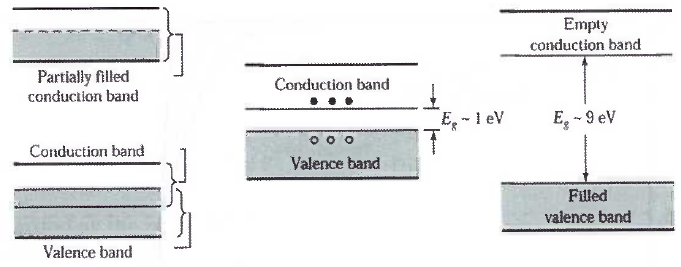
\includegraphics[width=0.7\textwidth]{ressources/bandgap.png}
\caption{Schematische Darstellung der Bandlücke eines Leiters (links), eines Halbleiters (mitte) und eines Isolators (rechts). \cite{SZE}}
\label{sze2}
\end{figure}

Für ein p-n-Übergang ist es nötigt ein Halbleiter-Material, meist Silizium, zusätzlich zu dotieren. Bei diesem Vorgang werden dem Halbleiter Fremdatome einer höheren oder einer niedrigeren Hauptgruppe hinzugefügt. Somit besitzt n-dotiertes Material einen Überschuss an Elektronen und p-dotiertes Material einen mangel an Elektronen, also effektiv einen Überschuss an Löchern, die als Quasiteilchen behandelt werden. 

Bei Kontakt entsteht der sogenannte p-n-Übergang. Dabei driften Elektronen in das p-dotierte und Löcher in das n-dotierte Halbleitermaterial. Durch die Rekombinationen in der Grenzschicht verbleiben ionisierte Atome, die ein elektrisches Feld entgegengesetzt zur Driftbewegung aufbauen und somit dem Drift weiterer freier Ladungsträger entgegenwirken, bis schlussendlich ein Gleichgewicht entsteht. In Abbildung \ref{sze3} ist die Fermienergie vor und nach Kontakt dargestellt.

\begin{figure}[H]
\centering
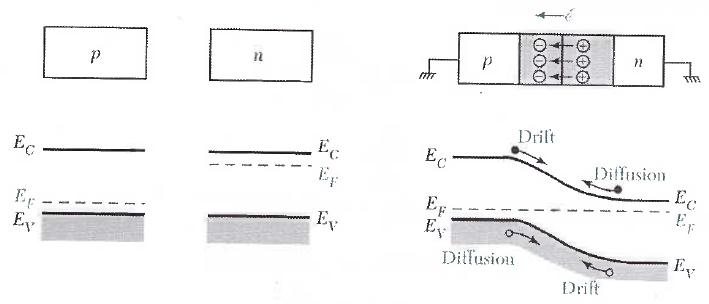
\includegraphics[width=0.7\textwidth]{ressources/junction.png}
\caption{Darstellung der verschobenen Fermienergie $E_F$ für ein n- und ein p-dotiertes Material (links) und bei Kontakt der beiden Materialien (rechts). \cite{SZE}}
\label{sze3}
\end{figure}

Die Ausdehnung der Depletionszone kann durch das Anlegen einer externen Spannung sowohl verkleinert also auch vergrößert werden. Bei Anlegen einer negative Spannung ($V<0$) an die n-dotierte Seite des Halbleiters, werden weitere freie Ladungsträger aus dem Material gezogen, wodurch sich die Depletionszone ausdehnt. Im Gegensatz dazu verkleinert sich die Depletionszone, wenn eine positive Spannung ($V>0$) angelegt wird. Die Depletionstiefe
\begin{align}
	d=\sqrt{\frac{2\epsilon\cdot(U_D-U)(N_D+N_A)}{q\cdot N_D\cdot N_A}}
\end{align} 
ist dabei sowohl von der Akzeptor- und Donatorkonzentration $N_{A/D}$, welche die Anzahl an eingebrachten Atomen zur n- und p-Dotierung pro Volumen beschreibt, als auch von der Dielektrizitätskonstante $\epsilon$ und der Elementarladung $q$ abhängig. Der Strahlungsrekombinationsstrom, der für die Emission von Photonen verantwortlich ist, steigt proportional zur Spannung. Somit ist es nach Abbildung \ref{sze4} vorgesehen, die Diode für diesen Versuch in Vorwärts-Richtung (V>0) zu betreiben.


\begin{figure}[H]
\centering
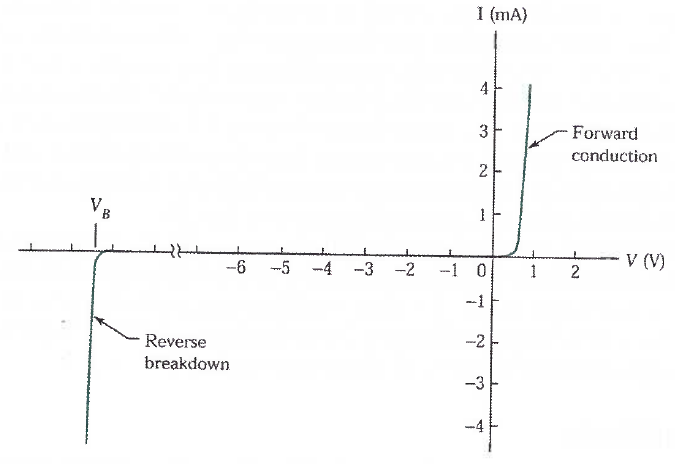
\includegraphics[width=0.5\textwidth]{ressources/IV.png}
\caption{Strom-Spannungs-Kennlinie für einen typischen Halbleiter. \cite{SZE}}
\label{sze4}
\end{figure}

\subsection{Dioden Laser}
Die in Kapitel \ref{sec:Bestandteile} angesprochenen essentiellen Komponenten eines Lasers, sind auch bei einem Diodenlaser zu finden. Der Halbleiter mit seinem p-n-Übergang wird als aktives Medium verwendet. Die entstehenden Bandlücke definiert die Wellenlänge der emittierten Photonen. Der angelegte Strom sorgt für den Pump-Prozess, da dieser Elektronen und Löcher einbringt und damit eine Art Besetzungsinversion zwischen dem Leitungsband und dem Valenzband hervorruft. Wie in Abbildung \ref{theo2} dargestellt, dient der Halbleiter selbst als Resonator und bildet einen optischen Wellenleiter. 

\begin{figure}[H]
\centering
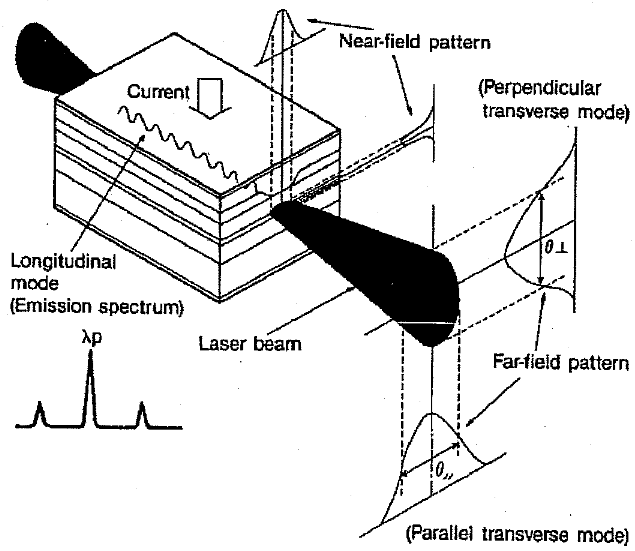
\includegraphics[width=0.5\textwidth]{ressources/Diode.png}
\caption{Schematische Ansicht der verwendeten Diode. \cite{skript}}
\label{theo2}
\end{figure}

Der entstandene Laser verlässt auf zwei entgegengesetzten Oberflächen die Diode mit einem elliptisch geformten Strahl, der sehr stark divergiert. Um die Sensitivität für andere Wellenlängen zu mindern, wird zusätzlich ein externer Resonator verwendet, auf den in späteren Kapiteln genauer eingegangen wird.

Für niedrige Ströme sind die Verluste im Medium so hoch, dass keine kohärente Strahlung stattfinden kann. Damit dominiert in diesem Bereich die spontane Emission mit einem breiten Spektrum, vergleichbar mit der Emission einer handelsüblichen LED. Wird der Grenzstrom $I$ (Threshold) überschritten, dominiert die kohärente Strahlung, wodurch der gewünscht Laserstrahl zustande kommt.

\section{TeachSpin Diodenlaser (Sanyo DL-2140-201S)} 

In den folgenden Kapiteln werden die Eigenschaften des verwendeten Lasers und der Aufbau des Experiments erläutert.

\subsection{Die Wellenlänge}
Die endgültige Wellenlänge des Lasers hängt stark von den verwendeten Komponenten und deren Konfigurationen ab. In der Abbildung \ref{theo3} ist die Laserausbeute, der sogenannte Net Gain gegen die Wellenlänge aufgetragen.

\begin{figure}[H]
\centering
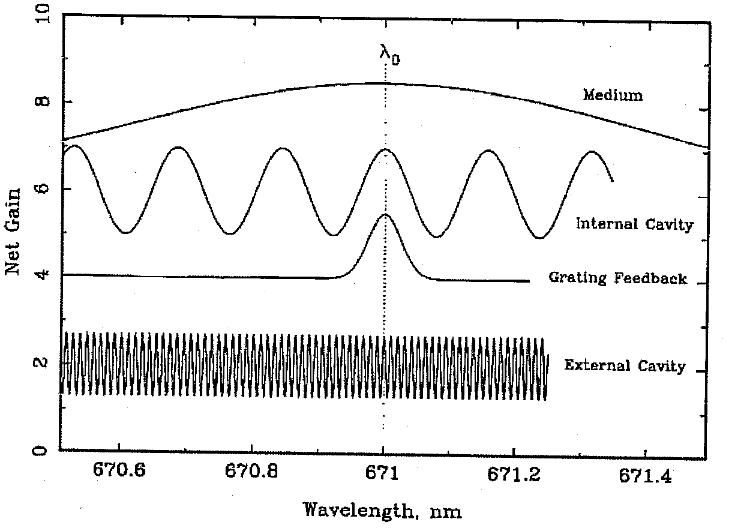
\includegraphics[width=0.8\textwidth]{ressources/net_gain.png}
\caption{Net Gain der einzelnen Laserkomponenten in Abhängigkeit der Wellenlänge. \cite{skript}}
\label{theo3}
\end{figure}

Das Spektrum des aktiven Mediums ist sehr breit und weißt eine hohe Ausbeute über einige Wellenlänge auf, ist dabei jedoch stark Temperatur und Stromabhängig. Wie in Abbildung \ref{fig:theo4} dargestellt, kommt es bei einem Temperaturanstieg zu einem Wellenlängenshift. Dieser wird durch eine Verkleinerung der Depletionszone bei hohen Temperaturen verursacht. Die Wellenlänge $\lambda_0$ kann ebenfalls durch eine Änderung des Diodenstroms verschoben werden. Die eingezeichneten Linien haben dabei eine Steigung von $\SI{200}{\mega\hertz\per\milli\volt}$ und spiegeln die umsetzbaren Wellenlängen wieder, da sich im Resonator nur eine diskrete Anzahl von stehende Wellen ausbilden kann. Somit existieren zwei Varianten die Wellenlänge der ursprünglichen Mode des Lasers zu verändern. In der späteren Durchführung wird hierfür der Strom der Diode verwendet, da dieses eine instantane Verschiebung verursacht im Gegensatz zu einer Temperaturänderung.

\begin{figure}
\centering
\begin{subfigure}{.5\textwidth}
	\centering
	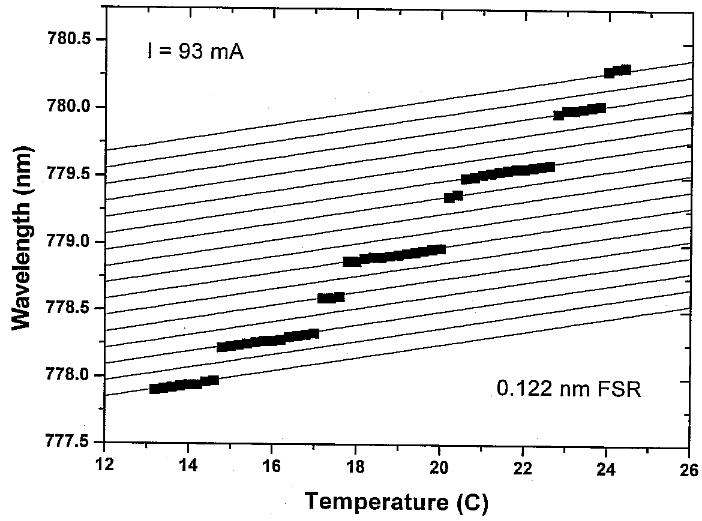
\includegraphics[width=0.7\textwidth]{ressources/Temp.png}
	\caption{In Abhängigkeit der Temperatur}
	\label{fig:Theorie1}
\end{subfigure}%
\begin{subfigure}{.5\textwidth}
	\centering
	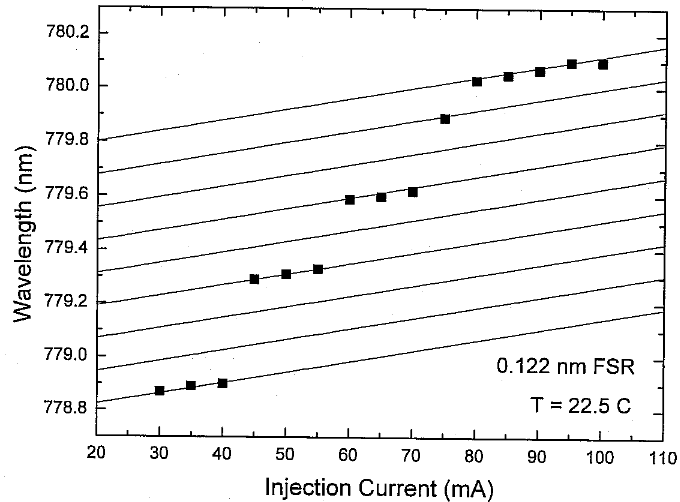
\includegraphics[width=0.7\textwidth]{ressources/Strom.png}
	\caption{In Abhängigkeit des Stroms}
	\label{fig:Theorie2}
\end{subfigure}
\caption{Darstellung des Wellenlängenshifts bei Änderung der Temperatur oder des Stroms. \cite{skript}}
\label{fig:theo4}
\end{figure}


Der Resonator hat eine Länge von $L=\SI{700}{\micro\meter}$ und einen Reflexionskoeffzienten von $n=3.6$. Der Abstand zwischen dem vom Resonator unterstützen Frequenzen wird auch als free spectral range bezeichnet und ist für den verwendeten Laser mit $\Delta\nu_{FSR}=\SI{60}{\giga\hertz}$ angegebenen. Mit Hilfe von Gleichung \ref{eq:1} ergibt sich somit der Abstand zwischen den Wellenlängen $\Delta\lambda_{FSR}=\SI{0.122}{\nano\meter}$.

Der Aufbau des Gitters erfolgt wie in Abbildung \ref{theo5} dargestellt.
\begin{figure}[H]
\centering
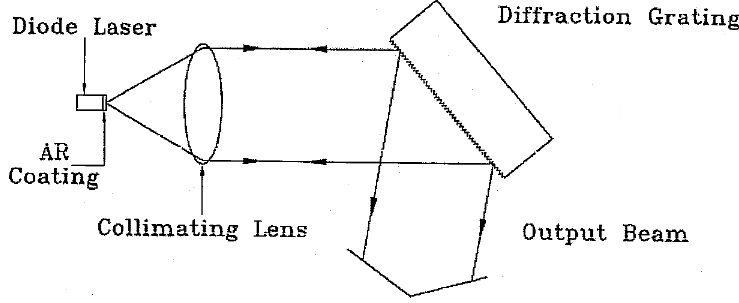
\includegraphics[width=0.7\textwidth]{ressources/Grating.png}
\caption{Positionierung des Gitters, welches die Länge des externen Resonators begrenzt. \cite{skript}}
\label{theo5}
\end{figure}

Dabei wird etwa $\SI{15}{\percent}$ des Lasers zurück in den Resonator reflektiert, welches zu einer Stabilisierung des Strahls führt. Analog wie zu einem Prisma wird nur unter einem bestimmten Winkel eine bestimmte Wellenlänge reflektiert, weshalb in Abbildung \ref{theo3} lediglich ein einzelnes Maximum dargestellt ist. Der Winkel des Gitters wird so gewählt, dass das Maximum erster Ordnung des Interferenzmusters reflektiert wird. Die Breite dieses Maximums
\begin{align}
	\Delta \nu= \nu/N
\end{align}
ist abhängig von der reflektierten Frequenz und der Anzahl der Gitterlinien, die vom Laserspot überdeckt werden. Mit den spezifischen Parametern ergibt sich hier eine Frequenzbreite von $\Delta \nu = \SI{70}{\giga\hertz}$.

Die Länge des externe Resonators kann durch einen Piezokristall modifiziert werden. Da der externe Resonator (L=$\SI{15}{\milli\meter}$) wesentlich größer als der interne Resonator (L=$\SI{700}{\micro\meter}$) ist, sind im Vergleich mehr Frequenzen zu realisieren. Aus diesem Grund ist das Signal in Abbildung \ref{theo3} hochfrequenter dargestellt. 

\subsection{Interne und externe Moden} 
In Abbildung \ref{theo5} ist erneut die Laserausbeute (Gain) gegen die Wellenlänge aufgetragen, jedoch unter verschiedenen Modenkonstellationen. 

\begin{figure}[H]
\centering
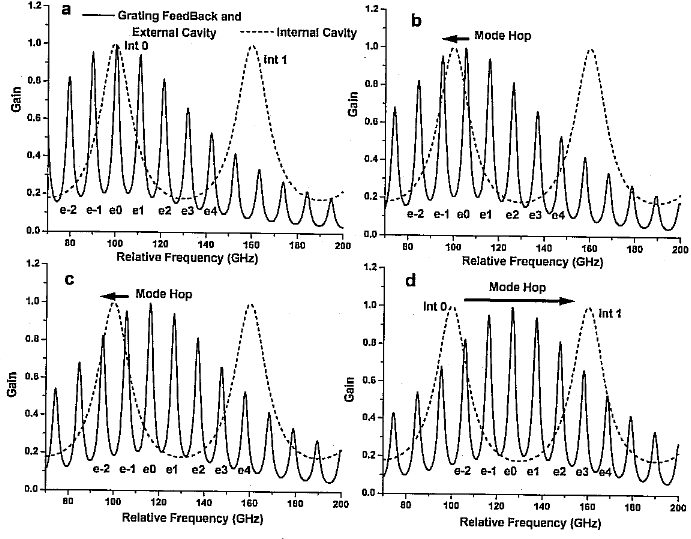
\includegraphics[width=0.8\textwidth]{ressources/Mode_Hop.png}
\caption{Grapfische Darstellung eines Mode-Hops. \cite{skript}}
\label{theo5}
\end{figure}

Die Maxima oder auch Moden des internen Resonators werden als Int0 oder Int1 und die Moden des externen Resonators e0, e1 oder e2 bezeichnet. In Abbildung a) stimmt die Wellenlängen des internen und des externen Resonators überein, wodurch diese Frequenz favorisiert wird. Durch eine Längenänderung des externen Resonators, verursacht durch die Ausdehnung des Piezokristalls, erfolgt eine Verschiebung der Wellenlänge, wie in Abbildung b) zu sehen. Bei dieser Ausrichtung wird keine einzelne Frequenz favorisiert, da sich die Moden e0 und e1 genau zwischen der Mode Int0 befinden. Erfolgt eine weitere Verschiebung der Frequenz wird die nächste Mode (siehe c) ) verstärkt. Dieser Vorgang des "Modenwechselns" wird auch als Mode-Hop bezeichnet. Ebenfalls der internen Modenwechsel wird als Mode-Hop bezeichnet.

Werden sowohl die Stromstärke als auch das Volumen des Piezokristalls simultan verändert, findet für beide Moden eine Wellenlängenverschiebung statt. Mit diesem Vorgehen ist es möglich ein kontinuierliches Frequenzspektrum mit dem Laser zu durchfahren, da kein Mode-Hop verursacht wird. Somit können verschiedene Anregungszustände eines Atoms untersucht werden, welches im folgenden anhand von Rubidium genauer diskutiert wird.

\subsection{Rubidium}

Mit dem nun geschaffenen kontinuierlichen Frequenzspektrum ist es möglich Absorptionslinien von Rubidium mit Hilfe der Lumineszenz zu beobachten. 

Lumineszenz tritt auf, wenn ein Photon im UV-Bereich ein Elektron anregt und  das Elektron somit in ein höheren Zustand übergeht. Relaxiert diese nach einer gewissen Zeit $\tau$ in den Grundzustand und emittiert dabei ein Photon im sichtbaren Spektrum, wird der Vorgang als Lumineszenz bezeichnet.

Das Aufspalten der Hyperfeinstruktur für $\ce{^{85}_{}Rb}$ und $\ce{^{87}_{}Rb}$ ist in Abbildung \ref{theo6} dargestellt. 

\begin{figure}[H]
\centering
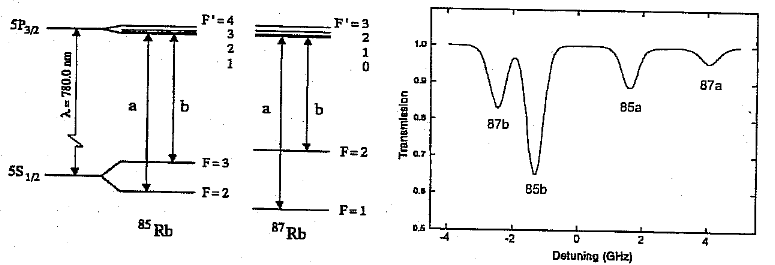
\includegraphics[width=0.8\textwidth]{ressources/Spektrum.png}
\caption{Durch ein Magnetfeld aufgespaltene Niveaus von $\ce{^{85}_{}Rb}$ und $\ce{^{87}_{}Rb}$. \cite{skript}}
\label{theo6}
\end{figure}

Für beide Isotope wird die Aufspaltung der Orbitale $5S_{1/2}$ und $5S_{3/2}$ betrachtet. Dabei spaltet das S-Orbital in zwei und das P-Orbital in vier Energieniveaus auf. Insgesamt sind vier Absorptionslinie zu beobachte. Der Grund dafür besteht darin, dass der Energieunterschied zwischen den Niveaus im P-Orbital im Gegensatz zum Unterschied im S-Orbital zu vernachlässigen ist. Bei der Betrachtung der Aufspaltung der beiden Grundniveaus fällt zusätzlich auf, dass der Abstand bei $\ce{^{87}_{}Rb}$ um etwa einen Faktor zwei größer ausfällt, als bei $\ce{^{85}_{}Rb}$. Dies hat zur Folge, dass der Übergang 87b im Vergleich zu den anderen Übergängen die niedrigste Frequenz und 87a die höchste Frequenz aufweist. Dazwischen befinden sich, aufgrund der geringeren Aufspaltung, die Übergänge von $\ce{^{85}_{}Rb}$.  

\newpage
\section{Justage und Durchführung}
In diesem Kapitel werden alle wesentlichen Schritte der Durchführung aufgelistet und die jeweilige Beobachtungen diskutiert. Es ist hier zu erwähnen, dass eine Speicherung eines Screenshots auf einem USB-Stick nicht möglich war, weshalb zur Dokumentation der Ergebnisse der Bildschirm des Oszilloskop mit einem Smartphone abphotographiert worden ist. 

\subsection{Stromminimierung}
Wie in Kapitel \ref{sec:diode} beschrieben, erzeugt die Diode bei zu geringem Strom inkohärente Strahlung, ähnlich einer LED. Um dieses zu beobachten wird eine IR-Indikatorkarte im Strahlengang des Lasers platziert. Mit einer UV-Kamera, die auf die IR-Karte fokussiert ist, kann nun der Laserspot über ein Bildschirm beobachtet werden. In diesem Teil der Durchführung muss eine UV-Kamera verwendet werden, da der Laserstrahl für das menschliche Auge nicht sichtbar ist, jedoch für die Kamera, da sie in diesem Wellenlängenbereich wesentlich sensitiver ist. Mit steigendem Strom $I$ steigt die Intensität linear an. Zu diesem Zeitpunkt weißt der Laserspot wohl definierte Grenze auf (siehe Abbildung \ref{fig:Theorie3}). Wird der 'Threshold' überschritten kommt es zur einer plötzlichen Intensitätsteigerung, die jedoch bei weiterem erhöhen des Strom erneut linear verläuft. An diesem Zeitpunkt ist der Laserspot und vor allem seine Grenzen als verschmiert oder diffus zu bezeichnen (siehe Abbildung \ref{fig:Theorie4}).

\begin{figure}
\centering
\begin{subfigure}{.5\textwidth}
	\centering
	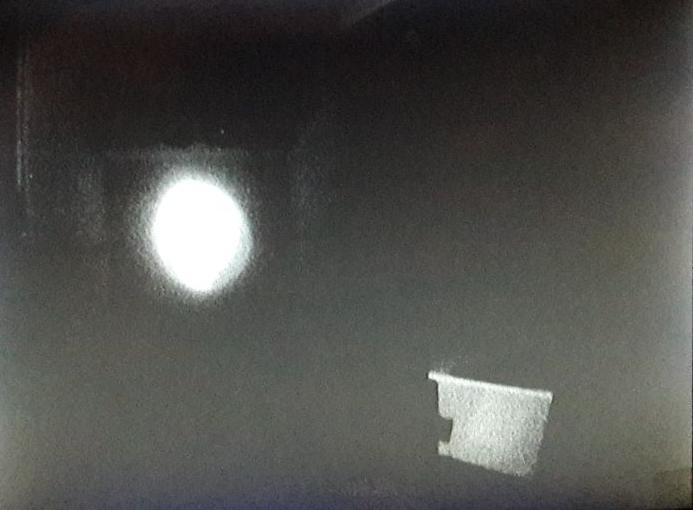
\includegraphics[width=0.6\textwidth]{ressources/inkohaerent.jpg}
	\caption{Inkohärente Emission}
	\label{fig:Theorie3}
\end{subfigure}%
\begin{subfigure}{.5\textwidth}
	\centering
	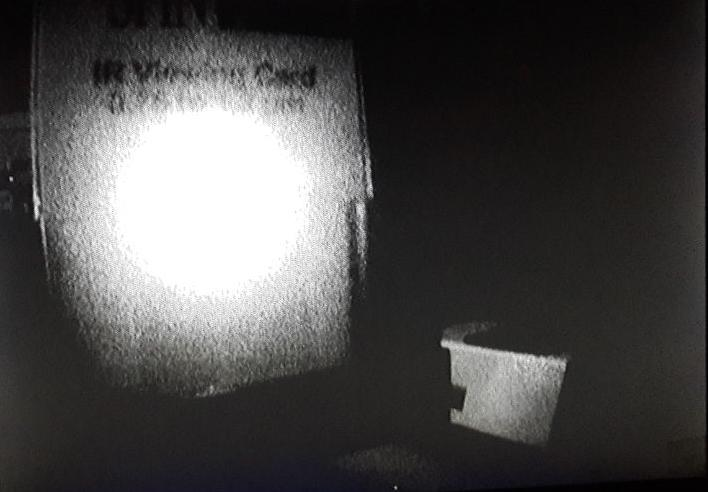
\includegraphics[width=0.6\textwidth]{ressources/kohaerent.jpg}
	\caption{Kohärente Emission}
	\label{fig:Theorie4}
\end{subfigure}
\caption{Darstellung der Emission des Lasers bei verschiedenen Stromstärken $I$.}
\label{fig:theo7}
\end{figure}


Für eine optimale Ausrichtung des Lasers ist der Strom zu minimieren. Dafür wird abwechselnd der Winkel des Gitters und die Länge des externen Resonators variiert bis der Laser kohärentes Licht emittiert. Danach wird der Strom so weit verringert, bis dieser sich unter dem Threshold befindet und die Prozedur erneut durchgeführt werden kann. Nach einigen Iterationsschritten ist somit der minimale Stromfluss erreicht. Um eine Aussage über den Threshold zu treffen, wird der Strom mit Hilfe des Oszilloskops einmal unter- und einmal oberhalb des Thresholds gemessen. Die Ergebnisse lauten:
\begin{align}
	U_{unter}=\SI{31.1}{\volt} \qquad \text{und} \qquad U_{über}=\SI{31.4}{\volt}
\end{align}
Für die beiden Ergebnisse wird der Mittelwert und die Standardabweichung bestimmt. Somit ergibt sich ein Threshold von $I=\SI{31.25 \pm 0.15}{\milli\ampere}$.

\subsection{Lumineszenz von Rubidium}
Nach der optimalen Justage wird nun die IR-Indikatorkarte aus dem Strahlengang entfernt, sodass der Strahl durch die Rubidium-Zelle propagiert. Diese ist mit gasförmigen Rubidium gefüllt und aufgeheizt. Die UV-Kamera wird seitlich neben der Zelle platziert, sodass die Lumineszenz im weiteren Verlauf gut beobachtet werden kann. Zunächst wird der Laserstrom erhöht. Daraufhin wird der Winkel des Gitters und die Länge des externen Resonators variiert, bis die richtige Wellenlänge (etwa 780$\:$nm) erreicht ist. Die Absorbtionslinie ist in Abbildung \ref{theo8} dargestellt. Es ist zusätzlich zu erwähnen, dass ein Filter und ein 50/50-Spiegel in dem Strahlengang platziert worden ist, um die Intensität des Lasers abzuschwächen.   

\begin{figure}[H]
\centering
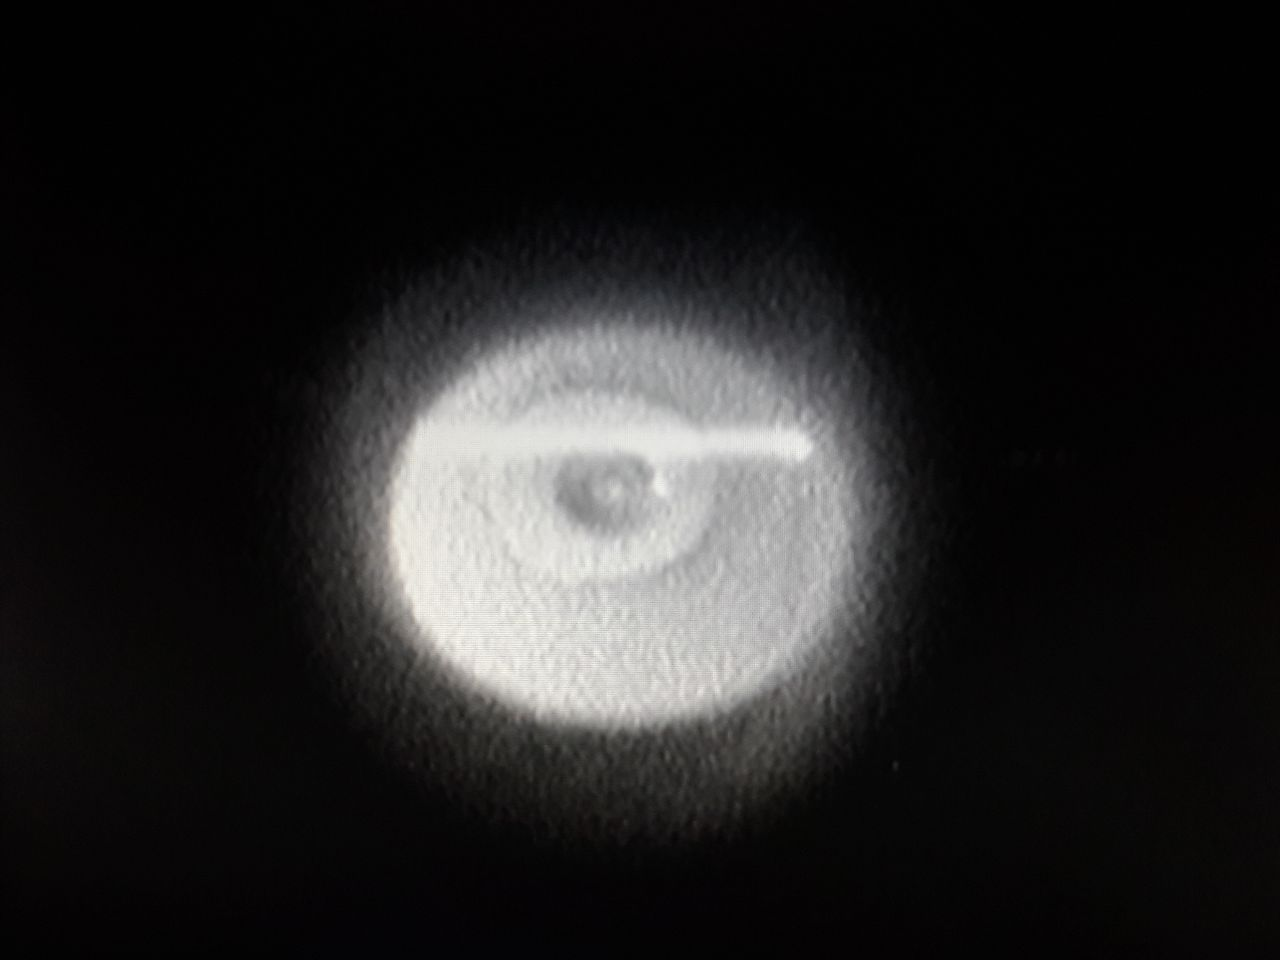
\includegraphics[width=0.7\textwidth]{ressources/Absorption.jpg}
\caption{Durch Lumineszenz hervorgerufene Absorptionslinie in Rubidium.}
\label{theo8}
\end{figure}


\subsection{Absortionsspektrum}
Das Ziel ist es nun, alle vier Absorptionslinie auf dem Oszilloskop sichtbar zu machen. Hierfür wird der Piezokristall verwendet, dessen Volumenausdehnung proportional zur angelegten Spannung ist. Somit kann die Länge des externen Resonators und dadurch die Wellenlänge des Lasers variiert werden. Angeschlossen an einen Rampengenerator wird die Expansion und Kompression des Kristalls mehrfach pro Sekunde durchgeführt. Die Folge ist ein schnelles Flackern in der Rubidium-Zelle. Mit einer Fotodiode, die hinter der Zelle platziert wird, kann die Intensität des transmittierten Lichts vermessen werden. Sowohl das Ausgangssignal, als auch das Signal des Rampengenerators wird auf das Oszilloskop gegeben, wodurch sich der Verlauf in Abbildung \ref{theo9} ergibt.

\begin{figure}[H]
\centering
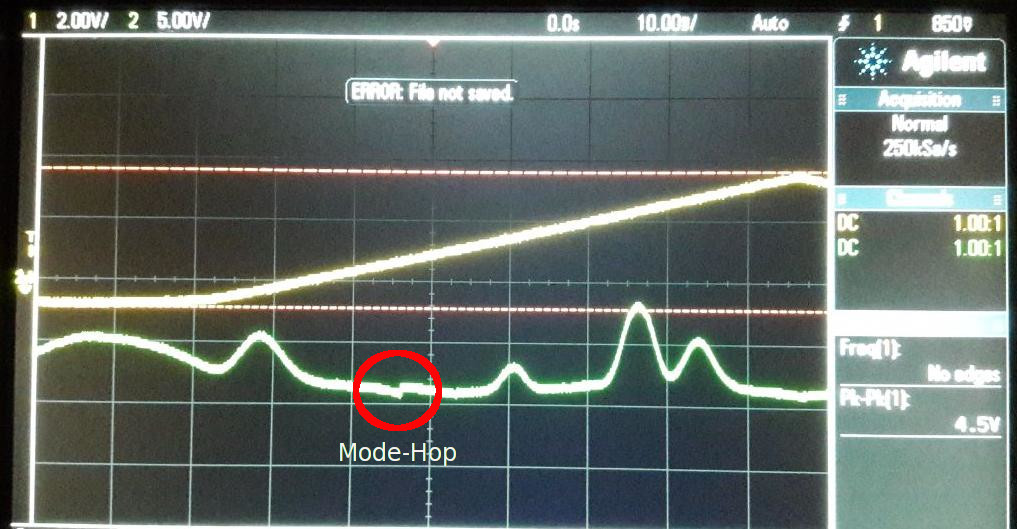
\includegraphics[width=0.7\textwidth]{ressources/Mode_Hop.jpg}
\caption{Absorptionslinie von $\ce{^{85}_{}Rb}$ und $\ce{^{87}_{}Rb}$ mit Mode-Hops.}
\label{theo9}
\end{figure}

Die hellgelbe Linie beschreibt die positive Flanke des Piezokristalls und somit seine lineare Volumenzunahme. Die grüne Linie zeigt zum einen vier Minima und zum anderen einen Mode-Hop, der gesondert in der Abbildung gekennzeichnet ist. Zur Vermeidung dieser Mode-Hops wird nun simultan die Länge des externen Resonators und der Laserstrom variiert, sodass ein kontinuierliches Spektrum durchlaufen werden kann. Das dadurch entstandene Messsignal ist in Abbildung \ref{theo10} dargestellt. Es sind deutlich die vier erwarteten Absorptionslinien zu sehen. Ebenfalls zu beobachten ist, dass das Messsignal der Fotodiode außerhalb der Absorptionslinien, nicht wie in der vorherigen Abbildung, konstant verläuft. Verursacht wird dieser stetige Anstieg durch die Steigerung des Laserstroms bei jeder positiven Flanke. Des weiteren ist eine minimale Oberwelle auf dem Signal zu beobachten, welche der Lichtquelle im Raum geschuldet ist. 

\begin{figure}[H]
\centering
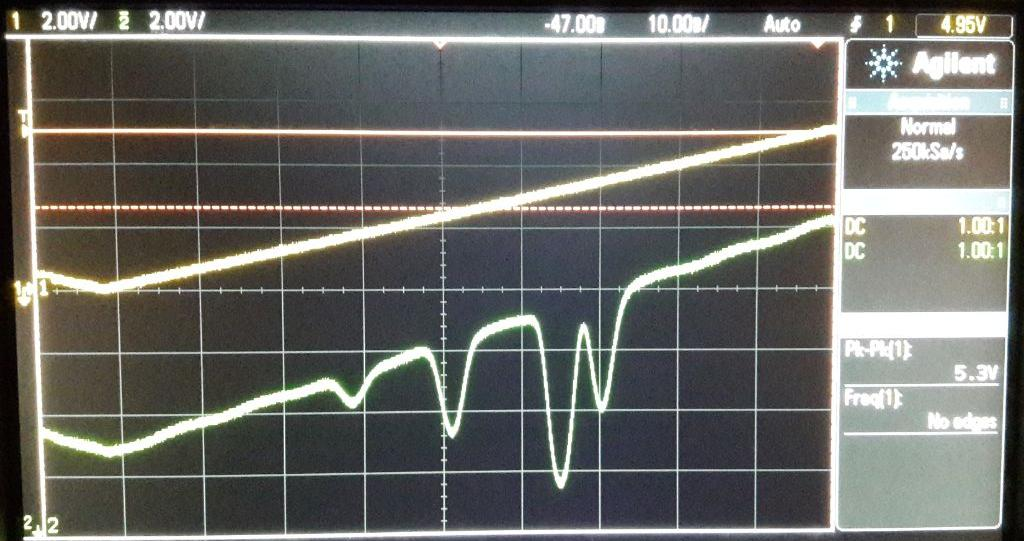
\includegraphics[width=0.7\textwidth]{ressources/Stromanstieg.jpg}
\caption{Absorptionslinie von $\ce{^{85}_{}Rb}$ und $\ce{^{87}_{}Rb}$ mit Intensitätsanstieg.}
\label{theo10}
\end{figure}

Für eine optimales Absorptionsspektrum, ohne Anstieg des Signals, wird dem Aufbau eine weitere Fotodiode hinzugefügt (siehe Abbildung \ref{theo11}). Diese misst, mit Hilfe des 50/50-Spiegels, das Signal direkt vor der Rubidium-Zelle. Somit erfasst die zweite Fotodiode, nur das linear steigende Signal ohne die Absorptionsmaxima. Für ein reines Absorptionssignal werden die beiden Signale von einander dividiert. Realisiert wird dieses mit dem folgenden Aufbau

\begin{figure}[H]
\centering
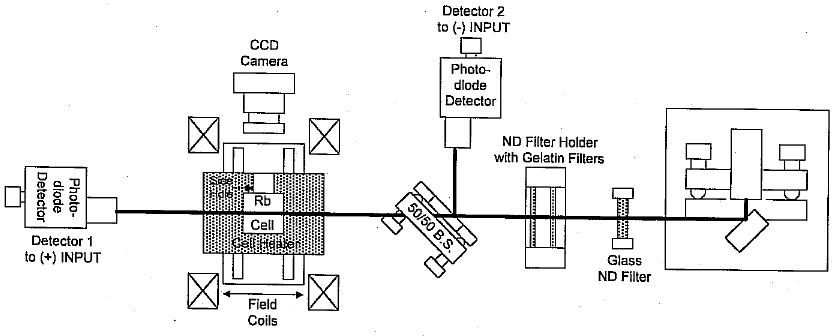
\includegraphics[width=0.8\textwidth]{ressources/Umbau.png}
\caption{Aufbau mit zusätzlicher Fotodiode. \cite{skript}}
\label{theo11}
\end{figure}

Dabei werden die Signal der beiden Fotodioden auf die beiden Eingänge gegeben. Durch die Drehknöpfe, die mit "Balance" beschriftet sind, kann das jeweilige Signal unterdrückt oder komplett hinzu geschaltet werden. Schlussendlich wird das dividierte Signal noch durch einen weiteren Drehknopf verstärkt, bevor es auf das Oszilloskop geführt wird. Auf diesem ist nun, wie in Abbildung \ref{theo12} dargestellt, das reine Absorptionsspektrum mit den vier Maxima und ohne Mode-Hops deutlich zu erkennen.

\begin{figure}[H]
\centering
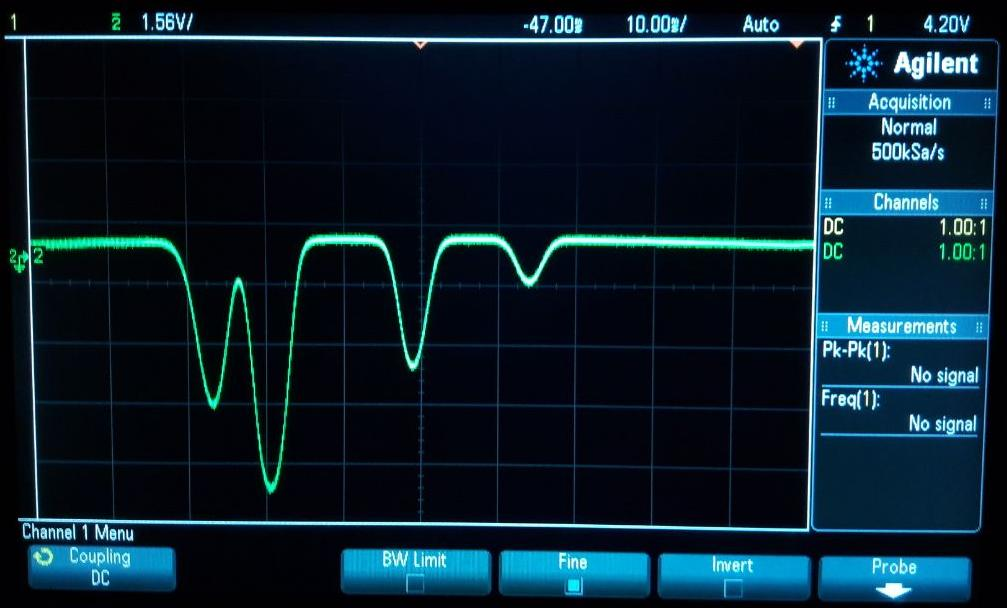
\includegraphics[width=0.7\textwidth]{ressources/final.jpg}
\caption{Absorptionslinie von $\ce{^{85}_{}Rb}$ und $\ce{^{87}_{}Rb}$}
\label{theo12}
\end{figure}
\newpage
\section{Zusammenfassung}

Zu Beginn der Durchführung wurde der Laserstrom für eine optimale Ausrichtung minimiert. Anschließend erfolgte eine genauere Justage der Wellenlänge, die mit einer Rubidium-Zelle durch Lumineszenz beobachtet werden konnte. Der Rampengenerator, mit dem die Länge des externen Resonators kontinuierlich variiert wurde, ist eine erste Erfassung des Absorbtionsignals gelungen. Die zu beobachtenden Mode-Hops wurde durch eine Veränderung des Laserstroms im Takt des Rampengenerators umgangen. Als letzter Punkt erfolgte die Bereinigung der Stromabhängigkeit des Signals durch ein zweites Fotodiodensignal, wodurch das reine Absorptionsspektrum von $\ce{^{85}_{}Rb}$ und $\ce{^{87}_{}Rb}$ aufgezeichnet werden konnte.        




% 2x2 Plot
% \begin{figure*}
%     \centering
%     \begin{subfigure}[b]{0.475\textwidth}
%         \centering
%         \includegraphics[width=\textwidth]{Abbildungen/Schaltung1.pdf}
%         \caption[]%
%         {{\small Schaltung 1.}}
%         \label{fig:Schaltung1}
%     \end{subfigure}
%     \hfill
%     \begin{subfigure}[b]{0.475\textwidth}
%         \centering
%         \includegraphics[width=\textwidth]{Abbildungen/Schaltung2.pdf}
%         \caption[]%
%         {{\small Schaltung 2.}}
%         \label{fig:Schaltung2}
%     \end{subfigure}
%     \vskip\baselineskip
%     \begin{subfigure}[b]{0.475\textwidth}
%         \centering
%         \includegraphics[width=\textwidth]{Abbildungen/Schaltung4.pdf}    % Zahlen vertauscht ... -.-
%         \caption[]%
%         {{\small Schaltung 3.}}
%         \label{fig:Schaltung3}
%     \end{subfigure}
%     \quad
%     \begin{subfigure}[b]{0.475\textwidth}
%         \centering
%         \includegraphics[width=\textwidth]{Abbildungen/Schaltung3.pdf}
%         \caption[]%
%         {{\small Schaltung 4.}}
%         \label{fig:Schaltung4}
%     \end{subfigure}
%     \caption[]
%     {Ersatzschaltbilder der verschiedenen Teilaufgaben.}
%     \label{fig:Schaltungen}
% \end{figure*}
